\nnsec{Results}

\nnsub{Adaptive Decision-Making Task for Head-Fixed Mice}

We trained head-fixed mice to perform a task requiring flexible sensorimotor mapping. In each trial, fluid-restricted mice were presented with one of two randomized auditory stimuli---either logarithmic frequency-modulated sweeps from 5 to 15 kHz (`upsweep') or from 15 to 5 kHz (`downsweep')---and were required to respond with a lick to the left or right port (Fig. \ref{fig:NN_fig1}a). A correct response was rewarded with 2 \si{\uL} of water, while an incorrect response resulted in white noise. Trials were organized into blocks (Fig. \ref{fig:NN_fig1}b), each with a distinct set of stimulus--response contingencies: `sound-guided' (upsweep-left; downsweep-right), `action-left' (upsweep-left; downsweep-left), and `action-right' (upsweep-right; downsweep-right). When performance reached a criterion of 85\% correct over 20 trials, a new block began with different contingencies. Sound and action blocks alternated, and no contextual cue was given to signal the block transition. Therefore, performance beyond the first block required flexible response selection and outcome monitoring. Mice were prepared for this task by initial training to an expert level on two-choice auditory discrimination; i.e., $\sim 30$ d on a task with only sound-guided trials. Here, we present data from mice with fewer than 6 sessions of experience in the adaptive decision-making task.

\begin{figure}[htbp]

\begin{center}
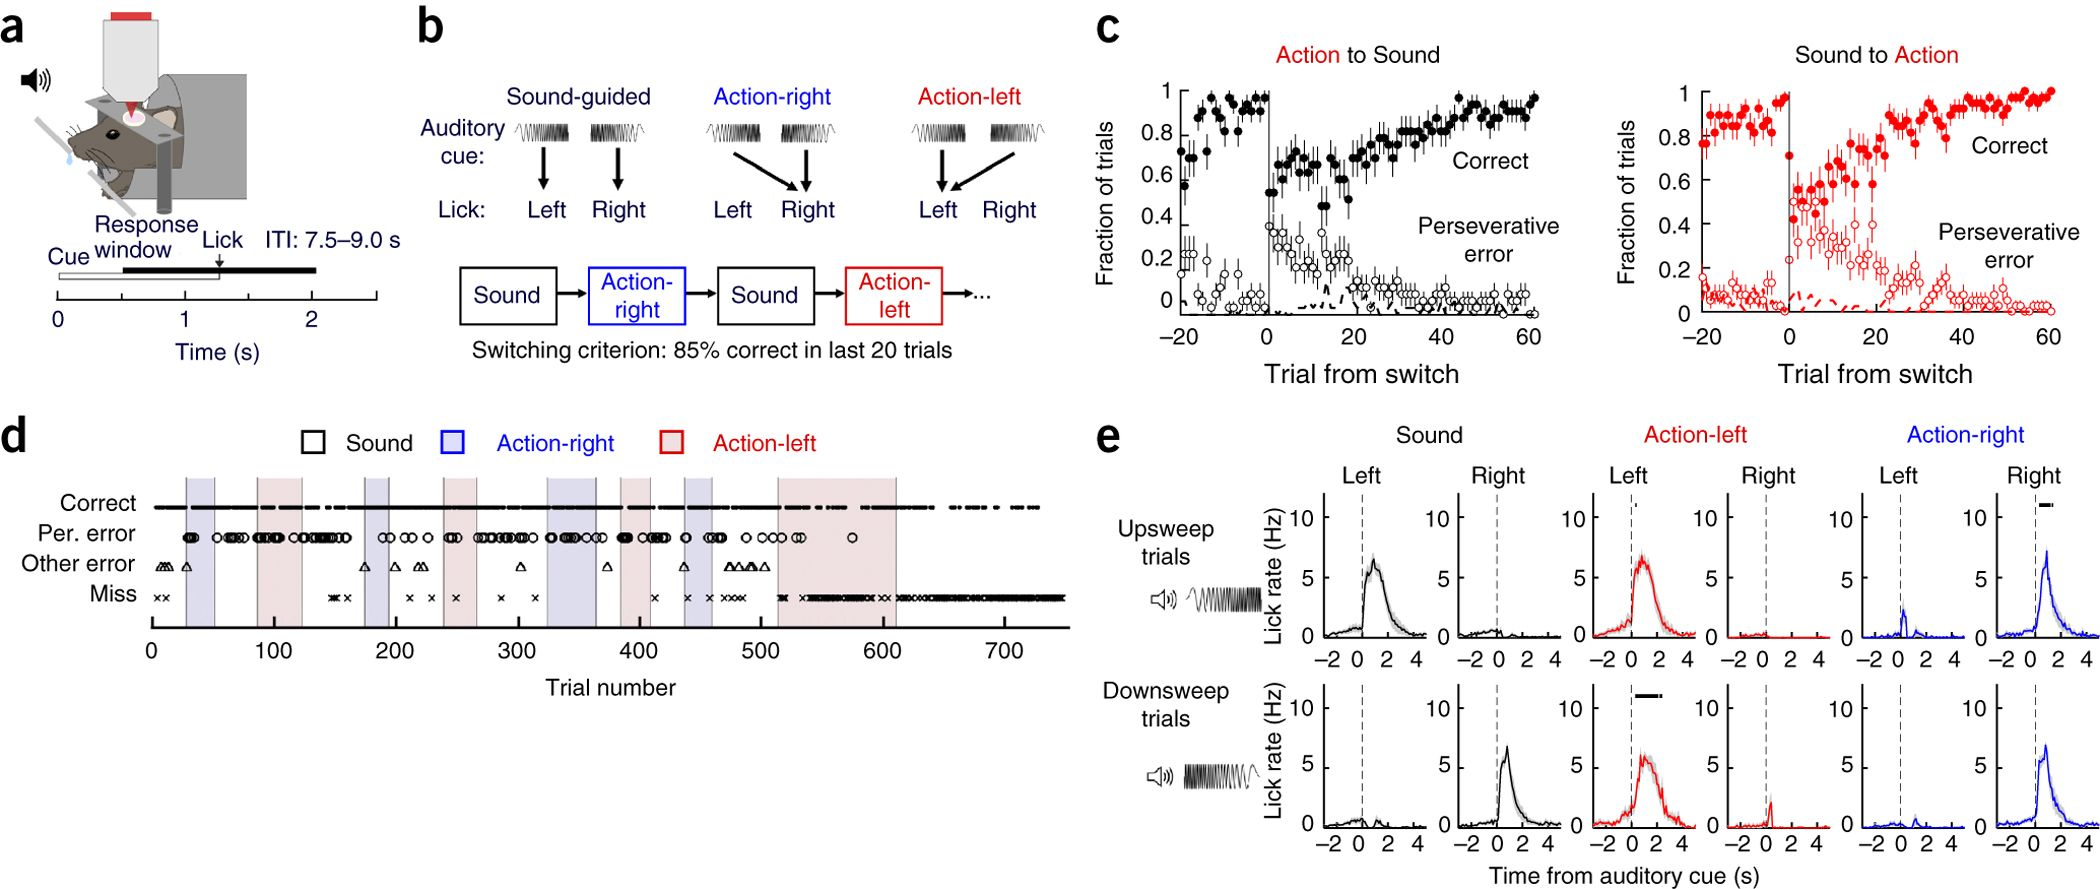
\includegraphics[width=\textwidth]{Figures/Chapter3/NN_fig1} 
\end{center}

\caption[Behavioral performance of head-fixed mice in an adaptive sensorimotor decision-making task]
{Behavioral performance of head-fixed mice in an adaptive sensorimotor decision-making task.
(a) Schematic of experiment. Each trial begins with an auditory cue. A response window starts 0.5 s after cue onset, during which the first lick is recorded as the response for that trial. Water reward is delivered contingent on a correct response. ITI, intertrial interval. (b) Schematic of stimulus–response mappings and block design. (c) Behavioral performance surrounding a block switch from action to sound (left) or sound to action (right). Filled circles, hit rate. Open circles, perseverative error rate. Dotted line, other error rate. $N=$ 33 action-to-sound switches and 38 sound-to-action switches. (d) Performance from one example behavioral session. Trial outcomes: correct (filled circles), perseverative error (open circles), other error (open triangles), or miss (cross). Vertical line, rule switch. (e) Left and right lick rates for upsweep or downsweep sound cues during all correct sound-guided (black), action-left (red) and action-right (blue) trials. For each choice direction, lick rates during action trials were compared to sound trials in 0.1 s bins; black bars, significant differences ($p<0.01$, paired t-test). All data presented as the $\mathit{mean}\pm\mathit{SEM}$. $N = 9$ sessions from 5 mice.}

\label{fig:NN_fig1}
\end{figure}

% \begin{FPfigure}

% \begin{center}
% 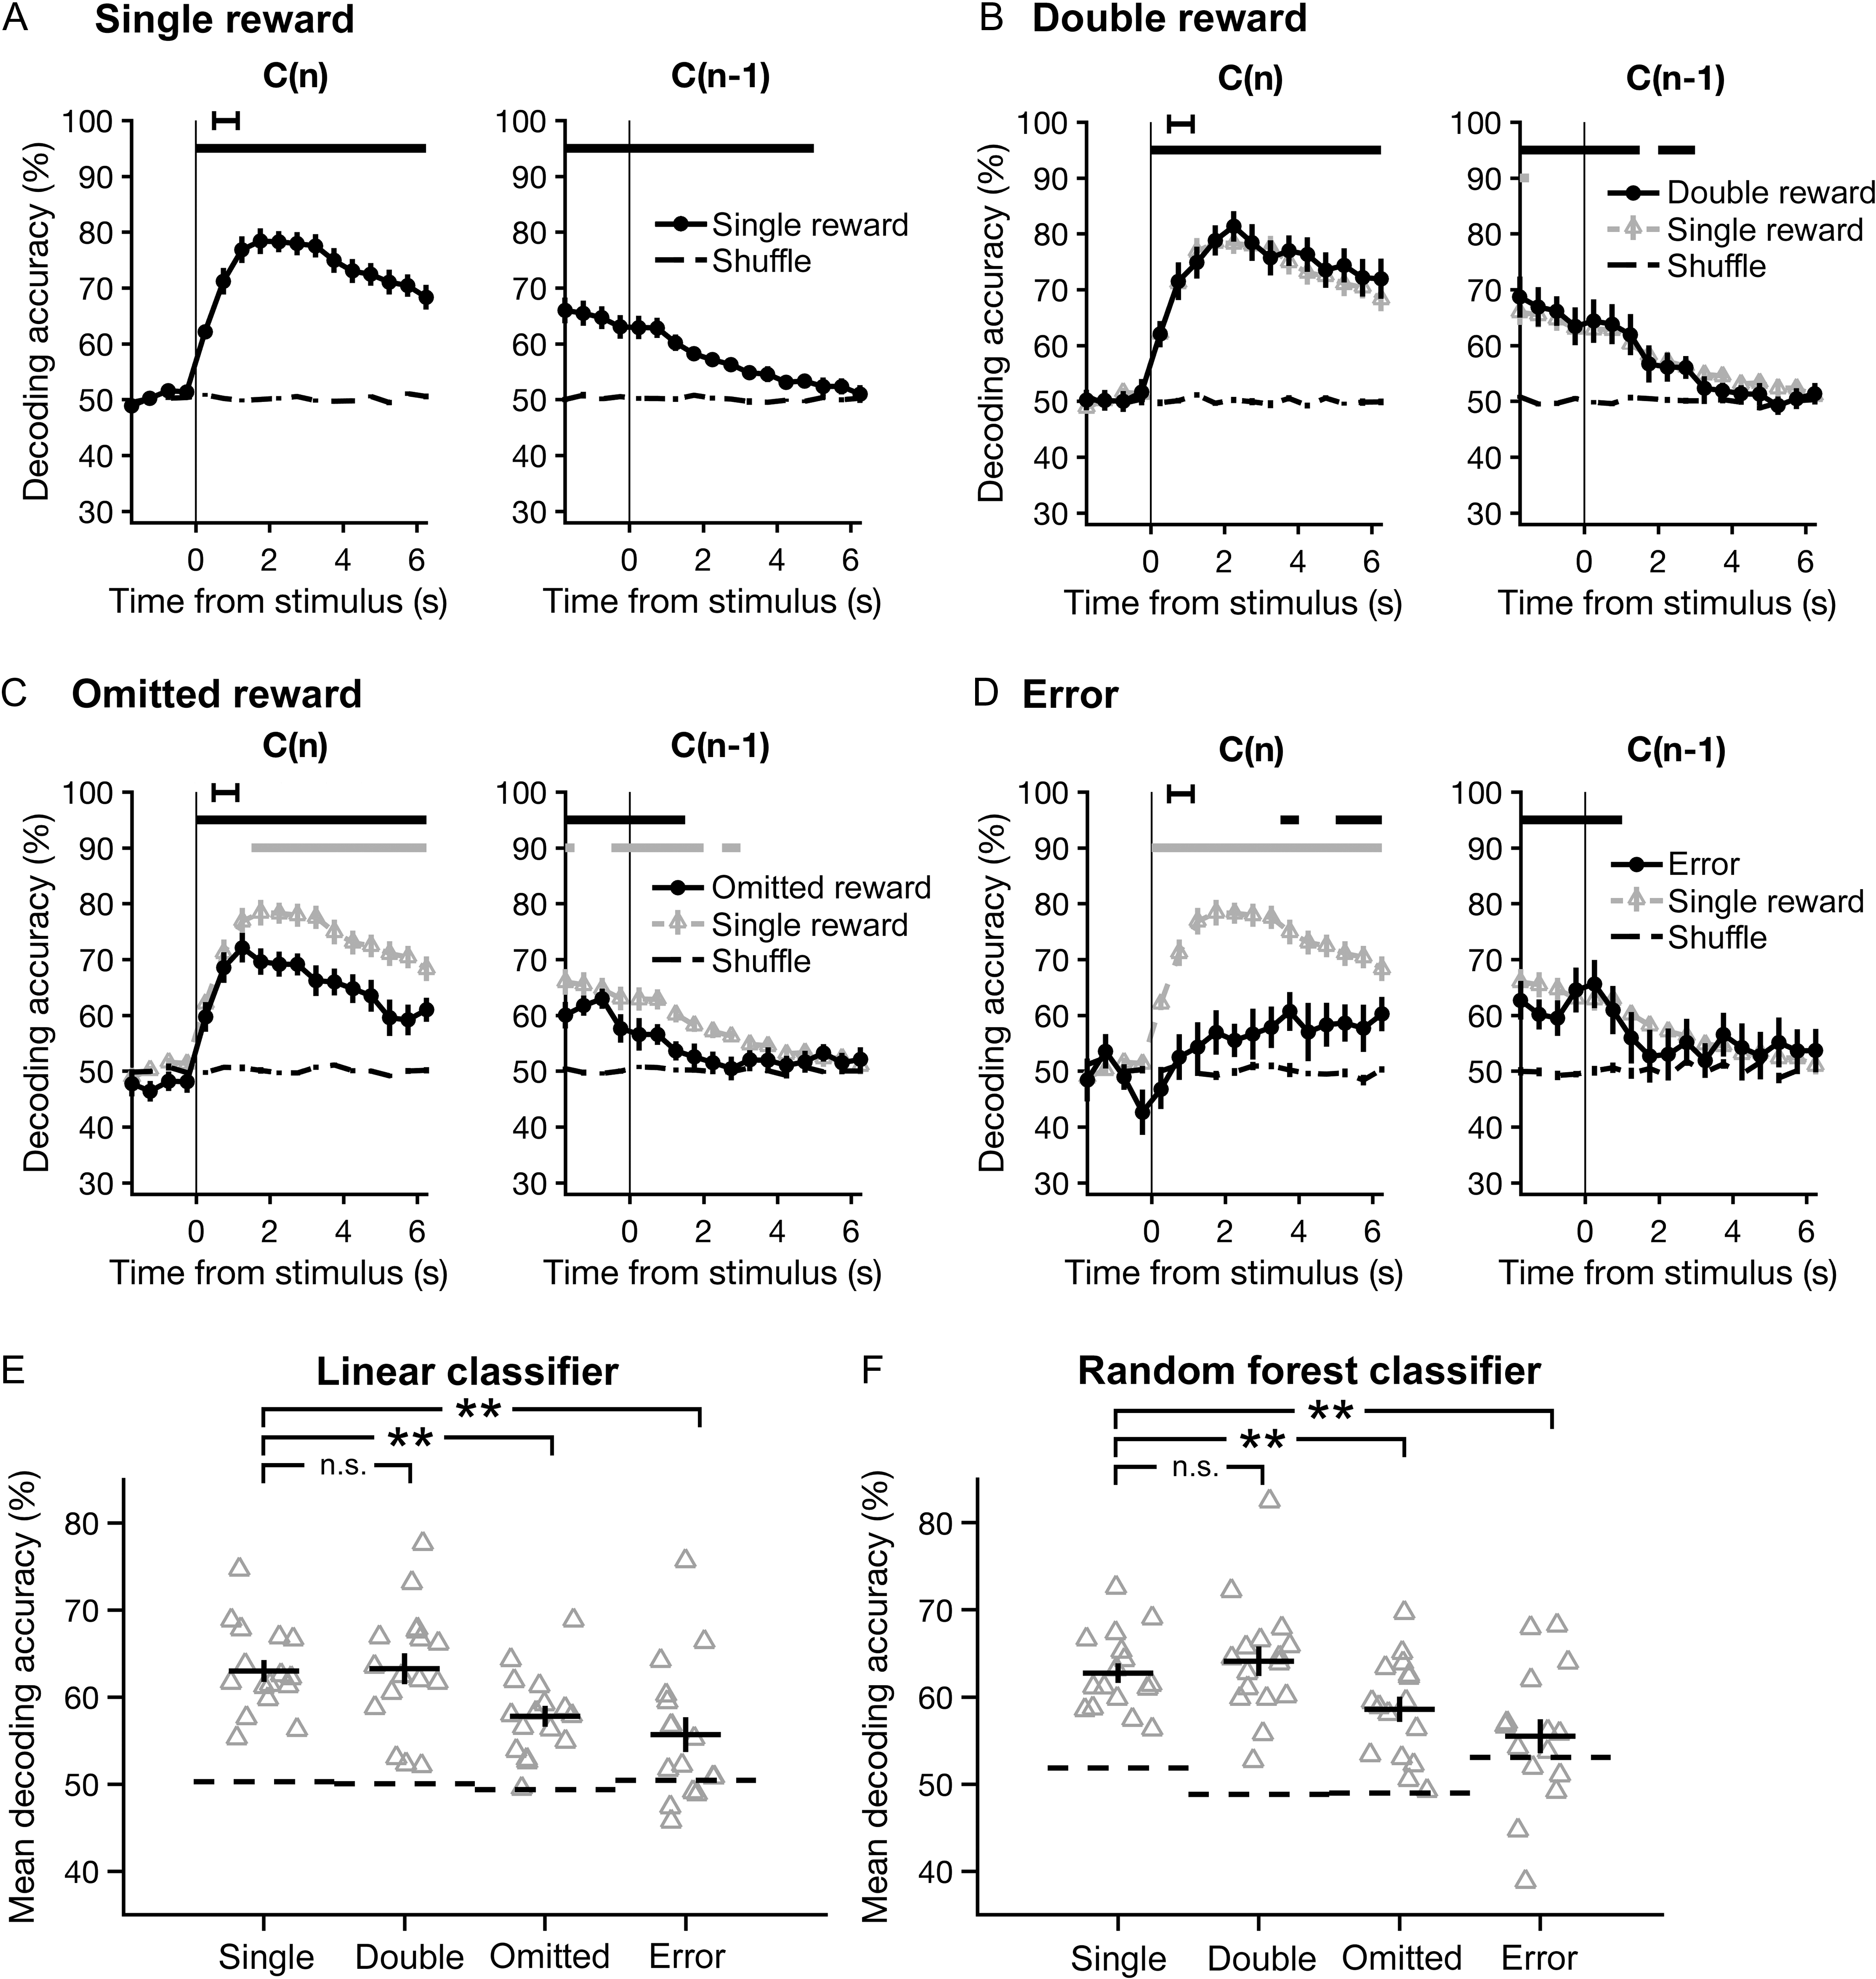
\includegraphics[width=\textwidth]{Figures/CC_fig6.png} 
% \end{center}
% \small{Figure \ref{fig:CC_fig6} Decoding accuracy diminished during omitted-reward and error trials. }

As expected, a switch in contingencies was associated with an immediate drop in correct response rate (Fig. \ref{fig:NN_fig1}c--d). Most incorrect responses were perseverative errors, indicating a failure to update response strategy for $\sim 20$ trials after the switch. We obtained concurrent calcium imaging and behavioral data during 9 sessions from 5 mice. On average, these mice performed $418 \pm 49$ trials per session, including $296 \pm 38$ rewarded trials and $9 \pm 1$ block switches ($\mathit{mean}\pm\mathit{SEM}$; range: 6–19 switches; Supplementary Fig. \ref{fig:NN_figS1}a). 

To quantify motor output, we calculated the mean lick rates and the time of first lick for different trial types. Overall, licks were tightly locked to the time of auditory cue during correct trials (Fig. \ref{fig:NN_fig1}e). For congruent trials (in which stimulus--response contingencies match), lick rates were indistinguishable across sound and action blocks. For incongruent trials (for example, left action for upsweep during sound block versus downsweep during action-left block), there was a noticeable difference in mean lick rates and an increased latency to first lick (Supplementary Fig. \ref{fig:NN_figS2}). Nevertheless, the major determinant of the distribution of lick times was response direction: i.e., whether the animal chose left or right (Fig. \ref{fig:NN_fig1}e). 

Additionally, we used video tracking to monitor whisker and hindpaw positions, and found that their movements also depended mostly on response direction (Supplementary Fig. \ref{fig:NN_figS3}). Therefore, although licks were the means for making operant responses in this head-fixed setup, mice performed more complex motor programs to indicate their choices.

\nnsub{Silencing M2 Selectively Impaired Shift to Sound-Guided Actions}
To determine whether frontal cortical activity is necessary for adaptive decision-making in our task, we used the GABA\textsubscript{A} receptor agonist muscimol to inactivate M2 bilaterally. Muscimol (5 mM, 46 nL per hemisphere) or saline vehicle was injected $\sim 1$ h before behavioral testing ($N=11$ mice; Fig. \ref{fig:NN_fig2}a). We injected low-molecular-weight fluorescein to estimate the extent of the affected region, which included M2 and part of cingulate cortex (Cg1), but not other neighboring regions (Fig. \ref{fig:NN_figS4}).
\begin{figure}[htbp]

\begin{center}
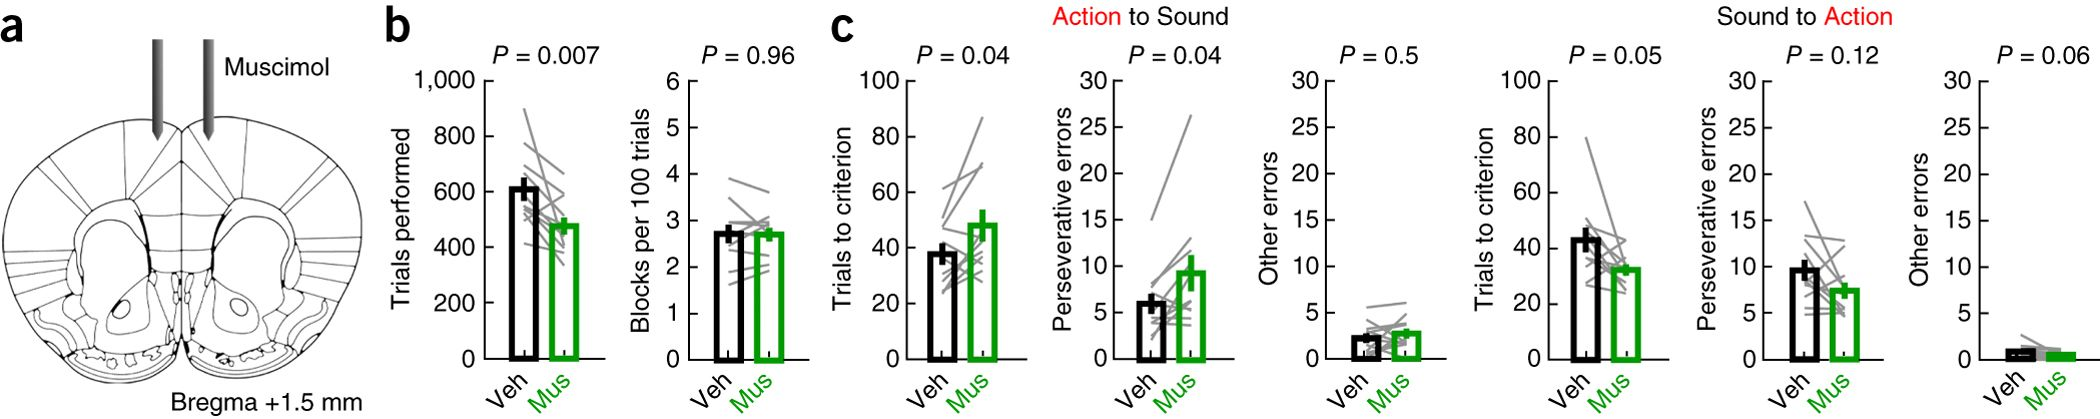
\includegraphics[width=\textwidth]{Figures/Chapter3/NN_fig2} 
\end{center}

\caption[Bilateral inactivation of M2 impaired adjustment to sound rule]
{Bilateral inactivation of secondary motor cortex (M2) impaired adjustment to sound-guided trials. (a) Schematic of experiment. (b) Task performance after bilateral infusion of saline vehicle (Veh) or muscimol (Mus) into M2. (c) Effects of muscimol infusion on action-to-sound and sound-to-action rule shifts. Gray lines, individual paired experiments. Bars, $\mathit{mean}\pm\mathit{SEM}$. Wilcoxon signed-rank test, action-to-sound: trials to criterion, $p = 0.042$, $W = 10$; perseverative errors, $p = 0.042$, $W = 10$; other errors, $p = 0.5$, $W = 24$. Sound-to-action: trials to criterion, $p = 0.054$, $W = 55$; perseverative errors, $p = 0.12$, $W = 51$; other errors, $p = 0.06$, $W = 46$. $N = 11$ mice.}

\label{fig:NN_fig2}
\end{figure}

Compared to controls, muscimol-injected mice performed fewer trials (Fig. \ref{fig:NN_fig2}b; saline: $608 \pm 42$, muscimol: $476 \pm 31$, $\mathit{mean}\pm\mathit{SEM}$; $p = 0.007$, $W = 62$, Wilcoxon signed-rank test), although there was no difference in the number of switches per 100 trials (saline: $2.7 \pm 0.2$, muscimol: $2.7 \pm 0.1$, $\mathit{mean}\pm\mathit{SEM}$; $p = 0.96$, $W = 34$). Inactivation had no effect on the timing or rates of lick motor output (Supplementary Fig. \ref{fig:NN_figS5}). 

Notably, separate analyses of sound and action blocks revealed selective impairments in the animals' ability to engage sound-guided actions, evidenced by a marked (55\%) increase in the number of perseverative errors per block (Fig. \ref{fig:NN_fig2}c; saline: $5.7 \pm 1.1$, muscimol: $8.9 \pm 1.9$, $\mathit{mean}\pm\mathit{SEM}$; $p = 0.042$, $W = 10$, Wilcoxon signed-rank test), and a greater number of trials to reach criterion (saline: $38 \pm 4$, muscimol: $48 \pm 6$, $\mathit{mean}\pm\mathit{SEM}$; $p = 0.042$, $W = 10$). Nevertheless, muscimol-injected mice eventually reached the criterion of $\ge 85\%$ correct, indicating that the transition to a high level of performance was slowed, but not blocked, by M2 inactivation. 

Silencing had the opposite effect on shifts into action blocks, during which the mice required fewer trials to reach criterion, although this effect fell short of statistical significance (saline: $43 \pm 4$, muscimol: $32 \pm 2$, $\mathit{mean}\pm\mathit{SEM}$; $p = 0.054$, $W = 55$). 

These results indicate a causal role for M2 in the flexible control of action selection. Additionally, the opposing effects of silencing are useful for understanding how the mouse performs the outlined task. One solution to the task would be to forget and relearn the relevant stimulus–response associations after each contingency change, as in a reversal task \citep{fusi2007neural}. This approach predicts symmetric changes in behavior following perturbations. An alternative approach would be to rely on these associations for sound-guided trials and then ignore them during action blocks to favor repeated selection of the same response. In this case, the mouse would perform the task by shifting the balance between conditional and unconditional means of responding. The asymmetric deficits observed in our experiments are consistent with the second approach and implicate M2 in the breaking of repetitive actions and biasing choices based on learned associations.

\nnsub{Imaging Task-Related Activity at Cellular Resolution in M2}
To characterize neural activity in layer 2/3 of M2, we injected an adeno-associated virus encoding GCaMP6s (AAV1-Syn-GCaMP6s-WPRE-SV40; Fig. \ref{fig:NN_fig3}a). GCaMP6s is a genetically encoded calcium indicator that exhibits a $\sim 25\%$ rise in fluorescence intensity per action potential in cortical pyramidal neurons \citep{chen2013ultrasensitive}. While mice performed the adaptive decision-making task, we used two-photon microscopy to record from $62 \pm 6$ cells per field of view ($\mathit{mean}\pm\mathit{SEM}$; range, 26–83 cells; $N = 9$ sessions from 5 mice; Fig. \ref{fig:NN_fig3}b). 
\begin{figure}[htbp]

\begin{center}
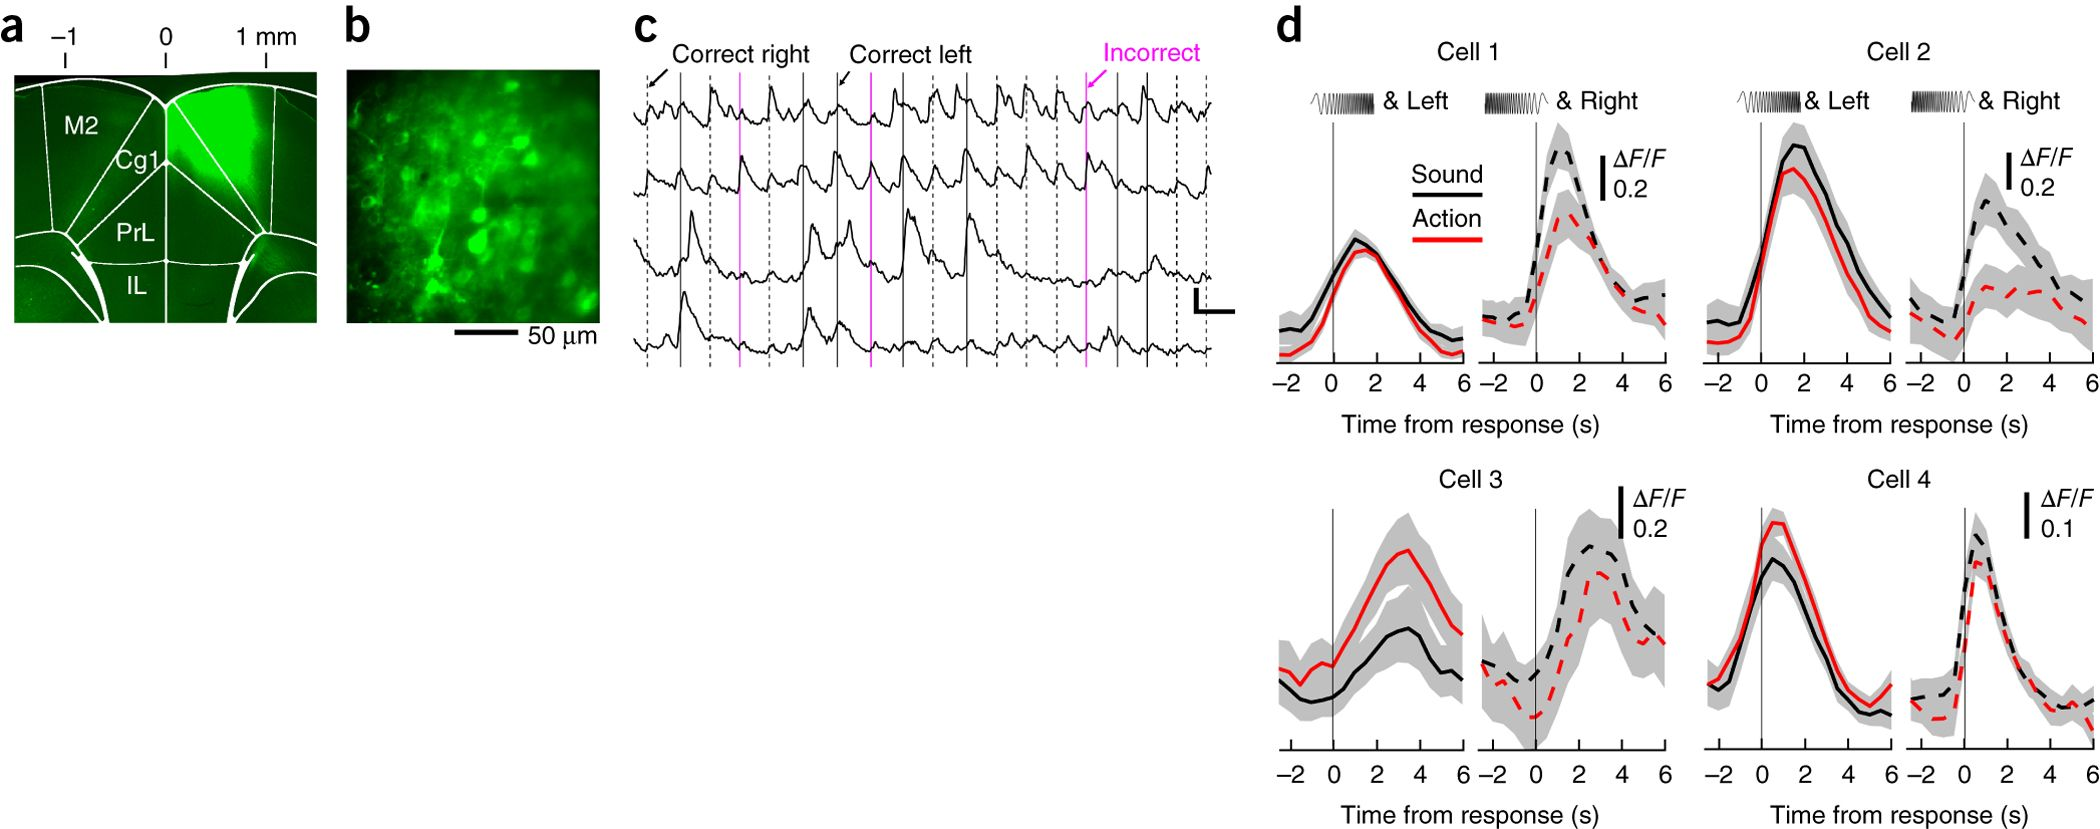
\includegraphics[width=\textwidth]{Figures/Chapter3/NN_fig3} 
\end{center}

\caption[Two-photon Ca$^{2+}$ imaging of task-related activity in M2]
{
Two-photon calcium imaging of task-related activity in M2.
(a) Example post hoc and (b) \emph{in vivo} two-photon images of GCaMP6s-expressing neurons in layer 2/3 of M2. PrL, prelimbic cortex; IL, infralimbic cortex. (c) Fractional fluorescence changes ($\Delta F/F$) in example M2 neurons during performance of sound-guided trials. Vertical lines indicate the time of response associated with correct left (solid black), correct right (dotted black), or incorrect (magenta) trials. Scale bars, 10 s and 100\% $\Delta F/F$. (d) Trial-averaged $\Delta F/F$ of four M2 neurons for correct left (solid line) and correct right (dotted line) responses in sound-guided (black) and action-guided (red) trials. Cell 1 corresponds to the top trace in c. Lines, mean. Gray shading, 95\% confidence intervals.
}


\label{fig:NN_fig3}
\end{figure}

Figure \ref{fig:NN_fig3}c shows four example M2 neurons with fluorescence transients ($\Delta F/F$) concurrent with responses during sound-guided trials. To examine how the use of conditional rules affects the activity of individual neurons, we averaged $\Delta F/F$ across correct trials for the congruent upsweep–left and downsweep–right conditions separately for sound and action blocks. Neural responses were diverse, even for neurons within the same field of view (Fig. \ref{fig:NN_fig3}d). During sound-guided trials, neurons could exhibit higher $\Delta F/F$ for specific associations---i.e., upsweep–left (cell 2) or downsweep–right (cells 1 and 3)---or have no preference (cell 4). The use of conditional rules modulated $\Delta F/F$ in some neurons (cells 1, 2 and 3) and in other cases had no effect (cell 4).

\nnsub{Neural Transition was More Rapid during Shift to Sound Rule}
The observed heterogeneity of neural responses opened the question of whether single-neuron activity in M2 reflects the components of an ensemble representation for specific task variables. If so, then population-level analyses might more effectively capture the content of such representations. Toward this end, we calculated population activity vectors from $\Delta F/F$ and used demixed principal component analysis (dPCA) \citep{machens2010functional,brendel2011demixed} to project the vectors in a reduced representational space (see Methods). Plotting these vectors over time generates trajectories describing the time-dependent evolution of ensemble activity during behavior. 

To determine how the ensemble activity evolved around block switches on a trial-by-trial basis, we calculated the Mahalanobis distances between population activity vectors of each trial and those of the 20 trials before the last or next block switch. Following a contingency switch, we found that the ensemble activity migrated away from the previous representational subspace toward a new subspace associated with the new rule (Fig. \ref{fig:NN_fig4}a). 
\begin{figure}[htbp]

\begin{center}
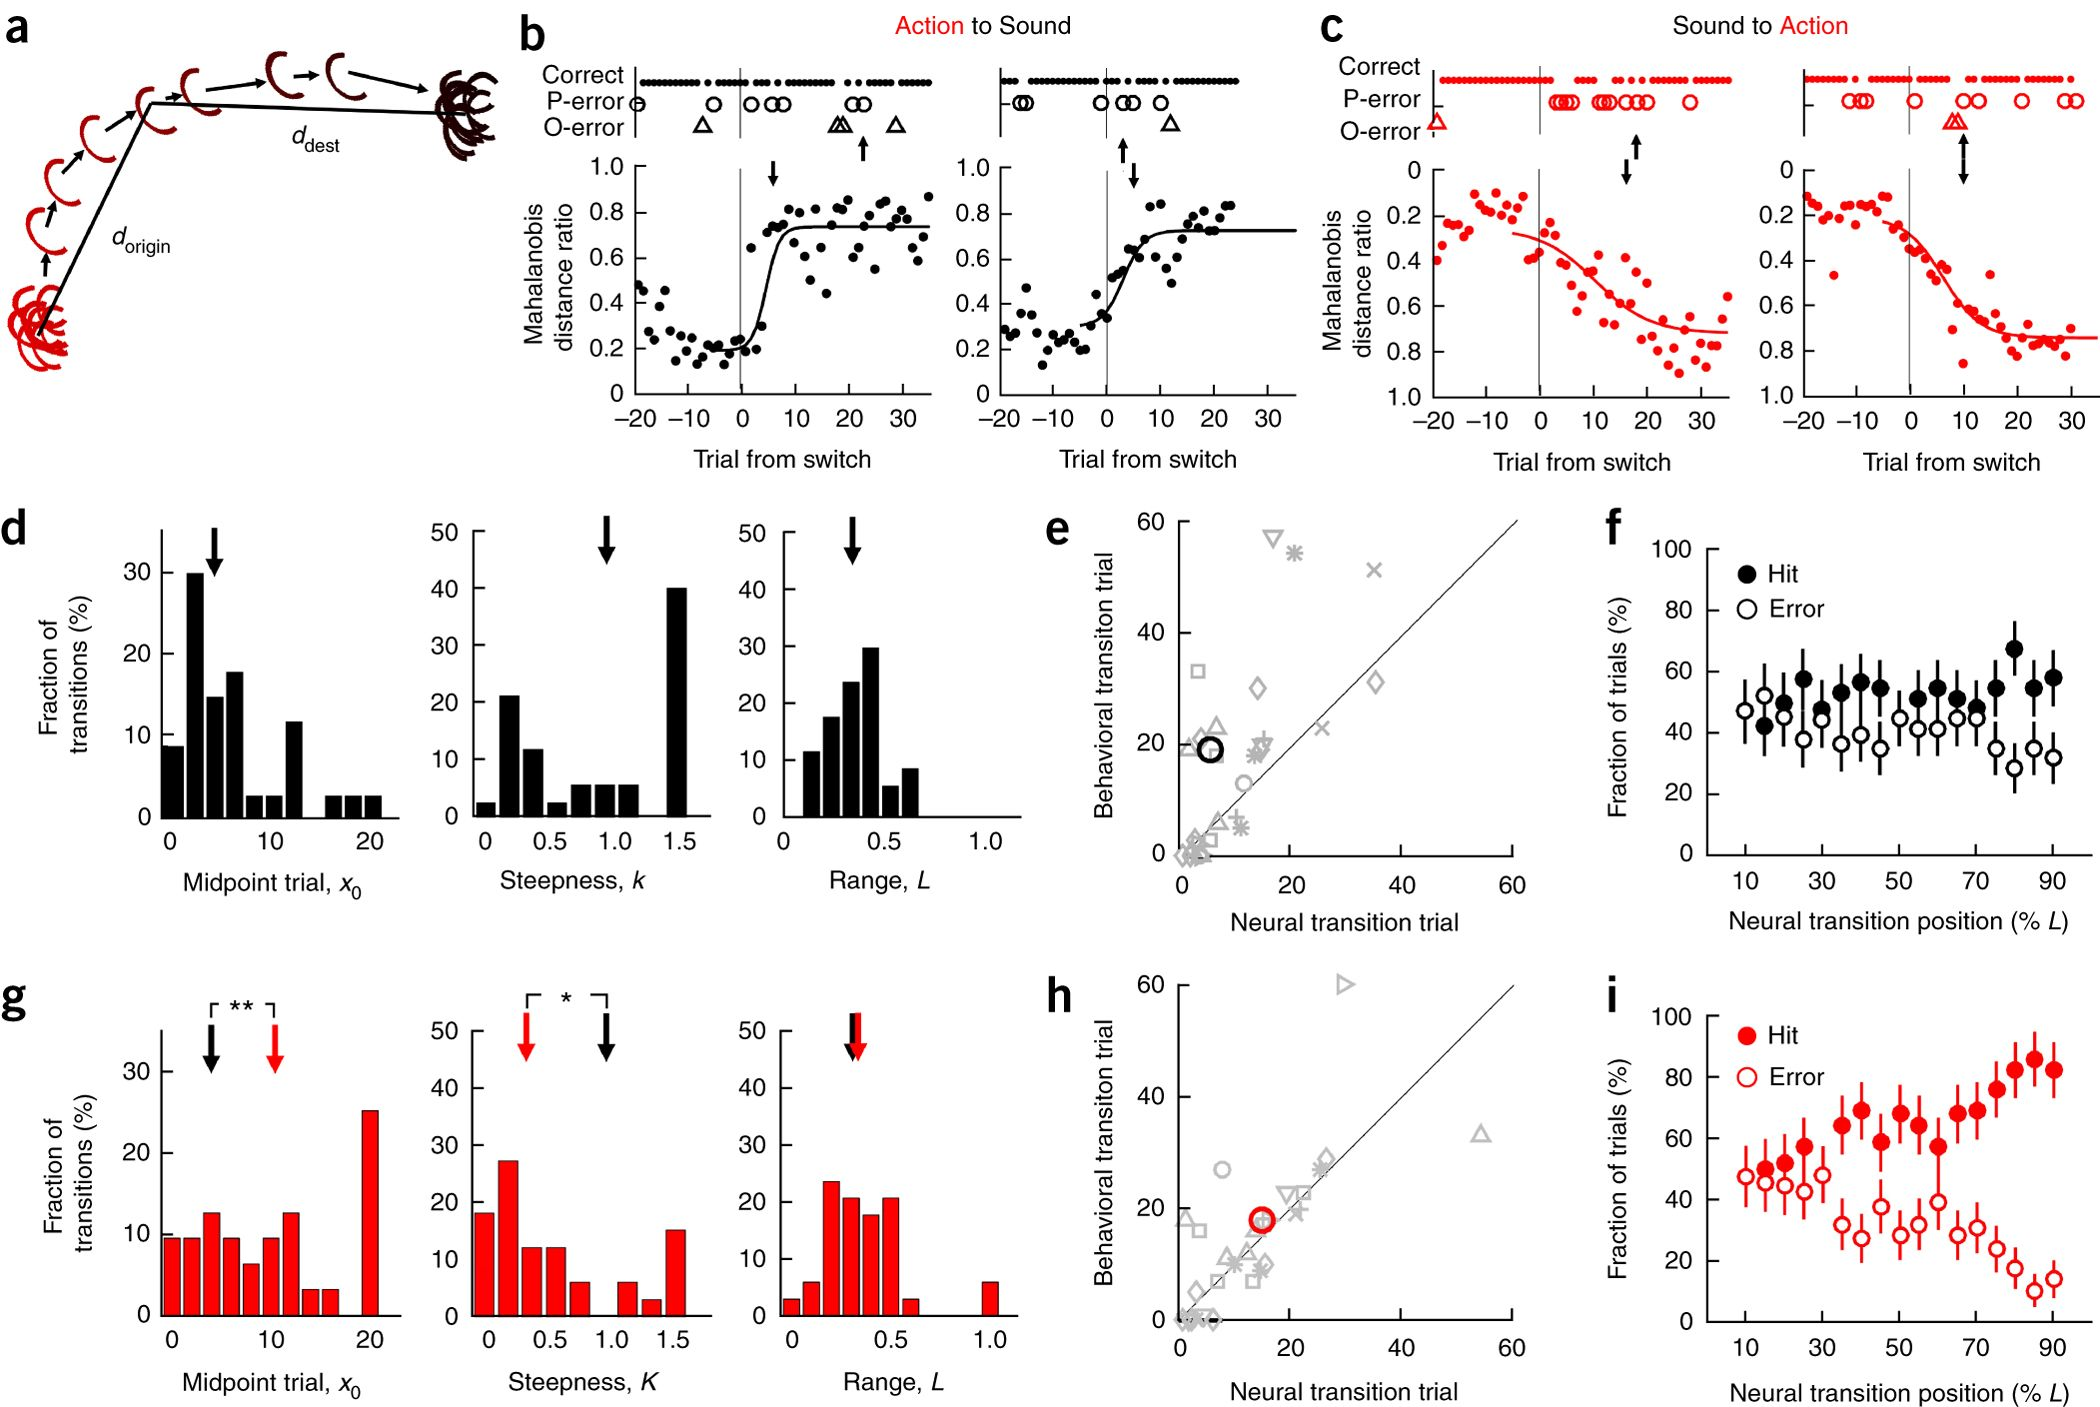
\includegraphics[width=\textwidth]{Figures/Chapter3/NN_fig4} 
\end{center}

\caption[Ensemble activity transitioned earlier and more abruptly following switch to sound rule]
{Transitions in ensemble activity occurred earlier and more abruptly following switch to sound rule. (a) Schematic illustrating ensemble activity dynamics around a block switch. Each curved line represents a single-trial neural trajectory deduced from Ca$^{2+}$-imaging data. When contingencies switch, neural trajectories move within the representational space. Trial-by-trial location of ensemble activity patterns was determined by calculating a ratio of Mahalanobis distances, $\frac{d_{origin}}{d_{origin} + d_{dest}}$, where $d_{origin}$ and $d_{dest}$ are the Mahalanobis distances from the neural trajectory of the current trial to those of the 20 trials pre-switch in the last and current blocks, respectively. (b) Two switches from action to sound blocks. Top, trial outcomes: correct (filled circles), perseverative error (P-error, open circles), and other error (O-error, open triangles). Bottom, trial-by-trial location of ensemble activity patterns. Dots, Mahalanobis distance ratios for individual trials. Lines, fit to logistic function. Up arrows, behavioral transition trials. Down arrows, neural transition trials. (c) Same as \emph{b} for two switches from sound to action blocks. Vertical axis is inverted for presentation purposes. (d) Parameters extracted by fitting action-to-sound neural transitions with the logistic function. Arrows, median values. (e) Neural transition trials plotted against behavioral transition trials (see Methods) for action-to-sound switches. Each symbol represents one block switch. Symbol shapes denote different sessions (see Supplementary Fig. \ref{fig:NN_figS6}). Large circle, median value. (f) Mean hit and error rates at the behavioral trial corresponding to specific neural transition locations as estimated by the logistic fit for each action-to-sound transition. Circles, $\mathit{mean}\pm\mathit{SEM}$. (g–i) Same as \emph{d--f} for switches from sound to action blocks; red arrows, median values; black arrows in \emph{g} shown for comparison with \emph{c}. Wilcoxon rank-sum test: for midpoint trial $x_0$, $p = 0.007$, $z = 2.70$; for steepness $k$, $p = 0.03$, $z = -2.17$; *$p < 0.05$; **$p < 0.01$. Difference in range $L$ was not significant (median $L$, sound: 0.36, action: 0.38; $p = 0.8$, $z = 0.28$). Rightmost bar of the histogram includes all instances above the range. $n = 33$ action-to-sound and 35 sound-to-action switches from 9 sessions from 5 mice.}

\label{fig:NN_fig4}
\end{figure}

Comparisons of the transition dynamics following a switch into conditional versus unconditional rules uncovered marked differences. Out of 33 action-to-sound and 38 sound-to-action transitions, 33 and 35 switches, respectively, could be fit with a logistic function to compare the onset and rate of shifts in population activity patterns (Fig. \ref{fig:NN_fig4}b--c). State transitions associated with the shift to sound-guided responses occurred after only several trials, much earlier than with shifts into repeated actions (Fig. \ref{fig:NN_fig4}d,g; sound: midpoint trial, $x_0 = 4.0$, action: $x_0 = 10.4$, median; $p = 0.007$, $z = 2.70$, Wilcoxon rank-sum test). Furthermore, breaking from repetitive to sound-guided responding involved transitions that were more abrupt (sound: steepness, $k = 1.02$, action: $k = 0.35$, median; $p = 0.03$, $z = -2.17$, Wilcoxon rank-sum test). These differences in neural dynamics were not due to behavioral differences, because in this set of experiments the number of trials to criterion was similar for the two rule types (sound: 39, action: 38, median; $p = 0.9$, $z = 0.09$, Wilcoxon rank-sum test; Supplementary Fig. \ref{fig:NN_figS1}a). 

Overall, these results suggest that ensemble activity patterns in M2 shift earlier and more steeply when animals are required to abort repetitive actions and engage conditional associations to perform sound-guided behavior.

To what extent must population activity resemble the final ensemble state in order to improve behavior? To address this question, we performed two analyses to compare the timing of neural and behavioral transitions. In the first analysis, we defined `transition trials' for behavior (the number of trials to criterion minus the 20-trial duration of the sliding window used for assessing criterion) and neural ensemble activity (Mahalanobis distance ratio equaling 75\% L based on logistic fit; see Methods). Block-by-block paired comparisons of neural and behavioral transition trials showed that ensemble activity in M2 shifted before the recovery of behavioral performance when adapting to conditional rules (Fig. \ref{fig:NN_fig4}e and Supplementary Fig. \ref{fig:NN_figS6}; $p = 0.003$, $z = -2.96$; Wilcoxon signed-rank test). By contrast, neural and behavioral changes occurred at around the same time for shifts to unconditional responding (Fig. \ref{fig:NN_fig4}h; $p = 0.19$, $z = 1.32$; Wilcoxon signed-rank test). 

We should note, however, that the definitions used for transition trials were arbitrary. Therefore, we performed a second, less biased analysis in which we determined the mean performance at the behavioral trial corresponding to a series of different neural transition locations. Compared with shifts to action trials (Fig. \ref{fig:NN_fig4}i), transitions to sound-guided trials were associated with hit and error rates that diverged later (Fig. \ref{fig:NN_fig4}f), indicating that behavioral improvement occurred later along the time course of neural transitions. 

Taken together, results of these two analyses suggest that when shifting to sound-guided actions, neural ensemble transitions in M2 are nearly complete before behavioral performance improvement can be detected.

\nnsub{Distinct Activity Patterns Accompanied Rule Implementations}
Our results indicated that rule shifts are associated with distinct transitions in network activity. This leads naturally to the question of what ensemble dynamics accompany successful rule implementation. We examined trajectories associated with correct responses in the 20 trials before the switch, when response strategies had stabilized ($\ge 85\%$ correct by task design). 

Figure \ref{fig:NN_fig5}a shows the trajectories of a 56-cell ensemble for left and right responses during sound-guided trials. The trajectories were initially indistinguishable and then diverged sharply after the animal made a response. Expanding this analysis to include action blocks revealed population activity patterns that occupied additional, distinct subspaces within the same representational space (Fig. \ref{fig:NN_fig5}b).
\begin{figure}[htbp]

\begin{center}
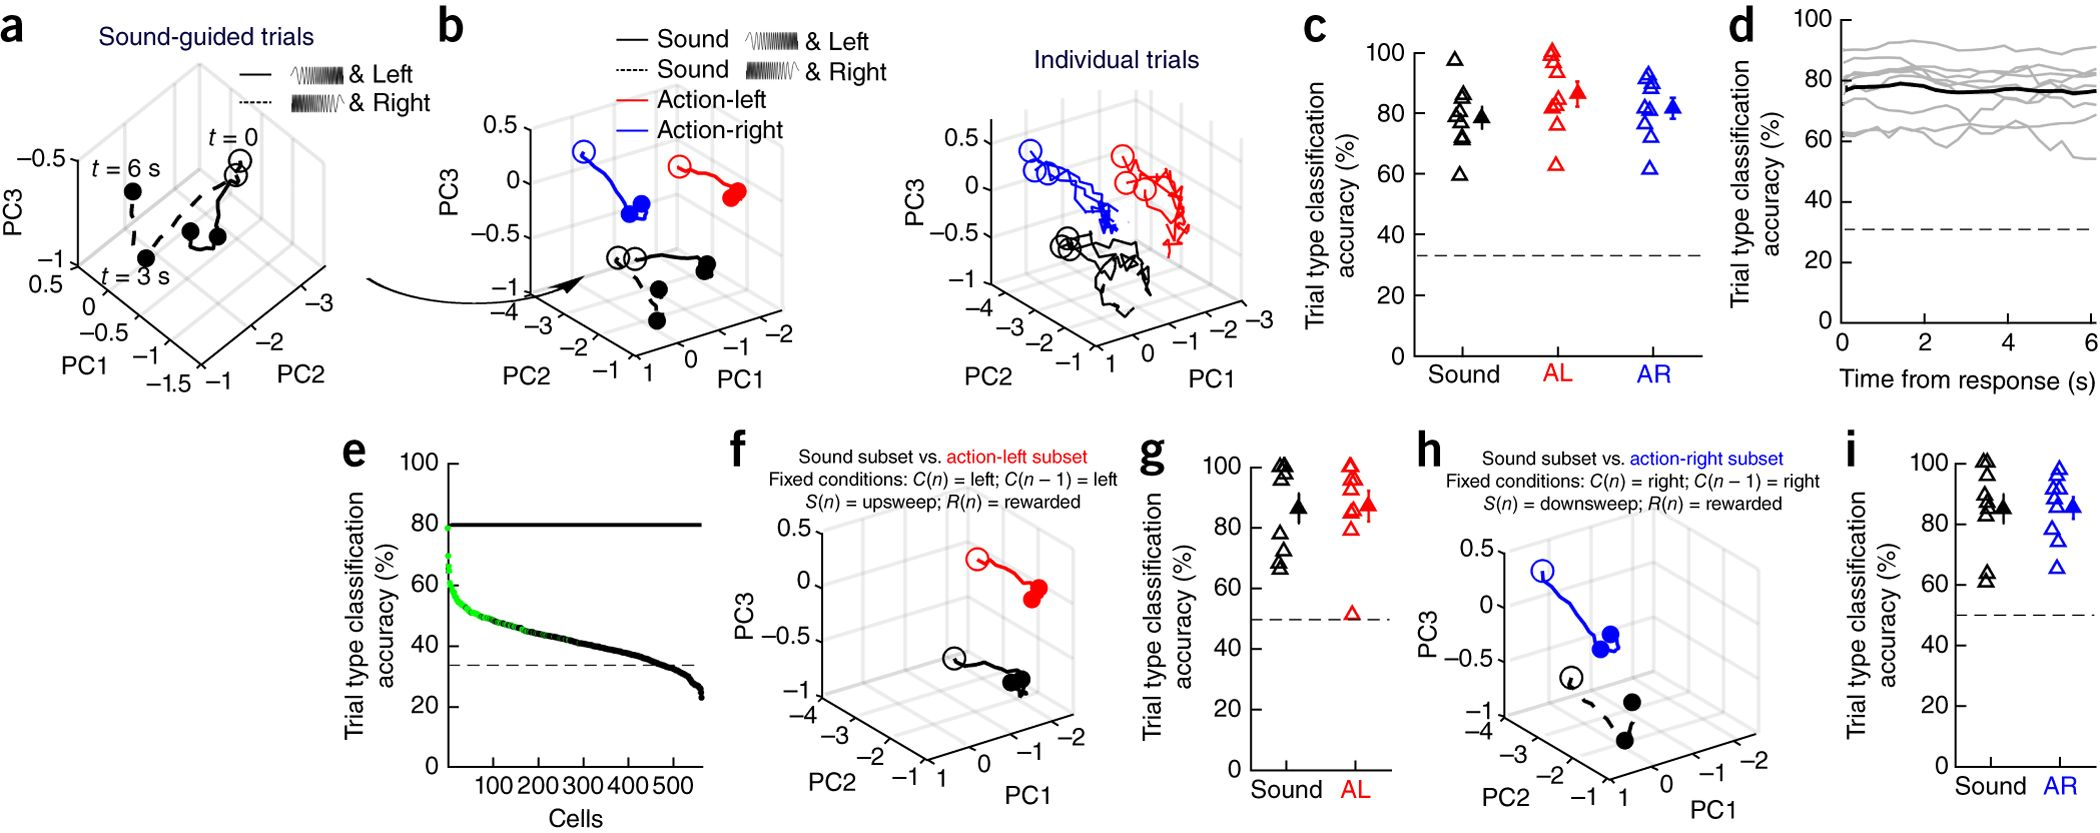
\includegraphics[width=\textwidth]{Figures/Chapter3/NN_fig5} 
\end{center}

\caption[Rule implementations were associated with distinct population activity patterns]
{
Rule implementations were associated with distinct population activity patterns.
(a) Neuronal circuit trajectories for 56 simultaneously imaged cells in one experiment. Trajectories were determined from trial-averaged $\Delta F/F$ for 44 correct left (solid line) and 59 correct right (dotted line) responses in sound-guided trials. Open circles, time of response $t_0$. Filled circles, 3 and 6 s after response. PC, principal component. (b) Same axes as \emph{a}, with additional trajectories from 51 correct action-left (red) and 51 correct action-right (blue) trials. Left, trajectories calculated using trial-averaged $\Delta F/F$. Right, three representative single-trial trajectories from each trial type. (c) Median accuracy of decoding trial type from individual population activity vectors. S, sound; AL, action-left; AR, action-right. Open triangles, individual experiments; filled triangles, $\mathit{mean}\pm\mathit{SEM}$; dotted line, chance-level accuracy. (d) Temporal dependence of ensemble decoding accuracy. Gray, individual experiments. Black, mean. Dotted line, chance-level accuracy. (e) Median accuracy of decoding trial type from fluorescence transients of single neurons. Green circles, trial-type-selective cells; i.e., 95\% percentile confidence intervals are above chance level of 33.3\%. Black circles, other cells. Black line, mean decoding accuracy using ensemble activity. Dotted line, chance-level accuracy. (f--g) Same as \emph{b--c} for trials in which stimulus was upsweep, choice was left, outcome was reward for the current trial and choice was left for the prior trial. Trial type could be decoded well above chance (sound: 87 ± 5\%, action-left: 88 ± 5\%; versus chance level of 50\%, $p = 7 \times 10^{-5}$, $7 \times 10^{-5}$, $t_8 = 7.50$, 7.52, one-sample t-test). (h--i) Same as \emph{b--c} for trials in which stimulus was downsweep, choice was right, outcome was reward for the current trial and choice was right for the prior trial. Trial type could be decoded well above chance (sound: $85 \pm 5\%$, action-right: $86 \pm 4\%$; vs. chance level of 50\%, $p = 7 \times 10^{-5}$, $8 \times 10^{-6}$, $t_8 = 7.54$, 10.01, one-sample t-test). $N = 9$ sessions from 5 mice.
}

\label{fig:NN_fig5}
\end{figure}

To quantify rule representations present in the population code, we asked how accurately block type could be predicted from individual population activity vectors. For each session, we constructed a classifier based on linear discriminant analysis (see Methods). Testing each classifier with five-fold cross-validation revealed that in all cases trial type could be decoded well above chance (Fig. \ref{fig:NN_fig5}c; sound: $78 \pm 3\%$, action-left: $86 \pm 4\%$, action-right: $82 \pm 3\%$; versus chance level of 33\%, $p = 1 \times 10^{-6}$, $1 \times 10^{-6}$, $5 \times 10^{-7}$; $t(8) = $ 13.2, 12.8, 14.3; one-sample t-test; $N = 9$ sessions). 

Repetition of this analysis using a moving window yielded high decoding accuracy at all times during a trial (Fig. \ref{fig:NN_fig5}d), consistent with a global shift in engagement of the network rather than a simple change in the processing of cue, action or outcome related signals. 

Next, we asked whether accuracy of the ensemble classifier could have been driven by a few highly rule-selective cells. When classifiers were trained on $\Delta F/F$ of individual cells, we found that 27\% of the cells could be used to decode block types at rates above chance; however, accuracy fell along a continuum and at levels below the accuracy of the ensemble (Fig. \ref{fig:NN_fig5}e). 

To ensure that the differences in trajectory and decoding accuracy were not due to simple sensory or motor parameters, we computed trajectories with matched stimulus, prior choice, current choice and outcome conditions. Analyses of these congruent trials, which differed only by rule, yielded similar results (Fig. \ref{fig:NN_fig5}f--i and Supplementary Fig. \ref{fig:NN_figS7}a--d). 

Taken together, these results indicate that the behavioral implementation of specific conditional and unconditional rules is associated with distinct network activity patterns in M2, such that population activity from any time during behavior can be used to decode task contingencies with high accuracy.

\nnsub{Activity Toggled between Rule-Related Patterns}
When animals solve trials with the same contingencies a second time, do M2 ensembles revisit similar activity patterns or does population activity migrate to a previously uncharted region of state space? Our task was well suited to address this question because blocks of the same trial type were presented multiple times within the same behavioral session. 

Figure \ref{fig:NN_fig6}a shows an example set of neural circuit trajectories for the first 12 trial blocks within one behavioral session, in which trajectories could be clearly grouped by block type and not by their temporal order. 
\begin{figure}[htbp]

\begin{center}
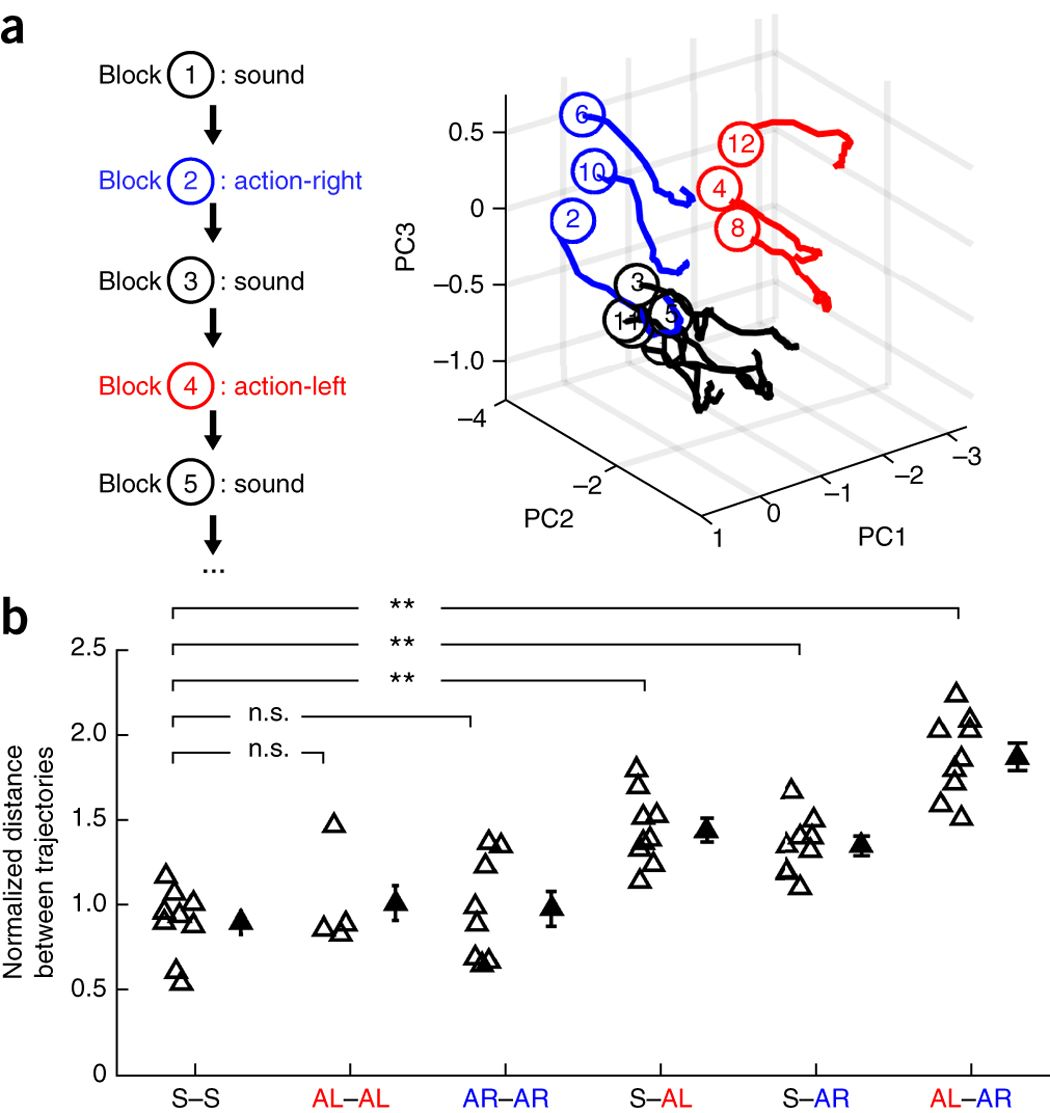
\includegraphics[width=8.7cm]{Figures/Chapter3/NN_fig6} %[width=11.4cm]
\end{center}

\caption[M2 ensembles revisited previous activity patterns upon re-exposure to corresponding rule]
{
M2 ensembles revisited previous activity patterns upon re-exposure to corresponding rule.
(a) Neural circuit trajectories calculated from trial-averaged $\Delta F/F$ for each trial block during one behavioral session. Circled numbers, temporal order in which trial blocks were presented. Open circles, time of response. Black, sound rule. Blue, action-right. Red, action-left. (b) Normalized distance between neural circuit trajectories from different trial types across all experiments (see Methods) for sound (S), action-left (AL) and action-right (AR). Open triangles, median distances from individual experiments. Solid triangles, $\mathit{mean}\pm\mathit{SEM}$. Wilcoxon signed-rank test: S--S vs. AL--AL: $p = 0.6$, $W = 3$; S--S vs. AR--AR: $p = 0.5$, $W = 13$; S--S vs. S--AL: $p = 0.004$, $W = 0$; S--S vs. S--AR: $p = 0.004$, $W = 0$; S--S vs. AL--AR: $p = 0.004$, $W = 0$; **$p < 0.01$. $N = 9$ sessions from 5 mice, except for AL--AL ($N = 4$) and AR--AR ($N = 8$) because mice did not perform enough switches to experience the same block type again in some sessions. **$p < 0.01$; n.s., not significant.
}

\label{fig:NN_fig6}
\end{figure}

To quantify the representational similarity of ensemble dynamics on a block-by-block basis, we calculated the mean Euclidean distances between all possible pairwise comparisons of trajectories within an experiment (see Methods). We found that neural circuit trajectories from blocks of the same type had a relatively small distance of separation and were similarly compact (Fig. \ref{fig:NN_fig6}b and Supplementary Fig. \ref{fig:NN_figS7}e--f; for sound (S), action-left (AL) and action-right (AR): S--S versus AL--AL: $p = 0.6$, $W = 3$; S--S versus AR--AR, $p = 0.5$, $W = 13$; Wilcoxon signed-rank test). By contrast, trajectories from different block types were represented by markedly different ensemble activity (S–S versus S–AL, $p = 0.004$, $W = 0$; S–S versus S–AR, $p = 0.004$, $W = 0$; S–S versus AL–AR, $p = 0.004$, $W = 0$; corrected $\alpha = 0.01$, Wilcoxon signed-rank test with Bonferroni correction). 

These results indicate that, during adaptive decision-making, M2 may toggle between distinct functional configurations as the animal repeatedly engages corresponding changes in task demands.

\nnsub{Comparison of Task-Related Neural Dynamics in M2, ALM and V1}
Next, we sought to determine whether the observed neural dynamics are specific to M2 or may also be found in other brain regions. For this purpose, we imaged neural ensembles in layer 2/3 of anterior lateral motor cortex (ALM; $65 \pm 6$ cells per field of view, $\mathit{mean}\pm\mathit{SEM}$; $N = 8$ sessions from 4 mice; Supplementary Fig. \ref{fig:NN_figS1}b) and primary visual cortex (V1; $57 \pm 7$ cells per field of view; $N = 4$ sessions from 2 mice; Supplementary Fig. \ref{fig:NN_figS1}c) to compare with the data from M2 ($62 \pm 6$ cells per field of view; $N = 9$ sessions from 5 mice). ALM has been implicated in motor planning and execution \citep{guo2014flow,li2015motor}; however, it is $\sim 1.5$ mm distant from M2, and the relationship between the two frontal cortical regions is not understood. V1 was chosen as a control region because the task was performed in the dark and involved no visual stimulus. 

Multiple linear regression analysis showed that M2 neurons robustly encoded not only the choice of the current trial, but also the choices of the two prior trials (Fig. \ref{fig:NN_fig7}a). A higher proportion of cells in ALM encoded the current choice; however, the signals decayed faster, resulting in weaker encoding of prior choices (Fig. \ref{fig:NN_fig7}b). Activity of M2 and ALM neurons could prefer either the ipsilateral or contralateral direction (Supplementary Fig. \ref{fig:NN_figS8}a--b), consistent with prior studies \citep{erlich2011cortical,li2015motor}. Unexpectedly, choice signals were also observed in V1 (Fig. \ref{fig:NN_fig7}c). Choice selectivity in V1 was relatively weak, and $\Delta F/F$ was almost always higher when animals made an ipsilateral choice (Supplementary Fig. \ref{fig:NN_figS8}c). Because choice signals in V1 were transient and animals performed the task in the dark, we conjecture that the selectivity might relate to corollary discharge. 

\begin{figure}[htbp]

\begin{center}
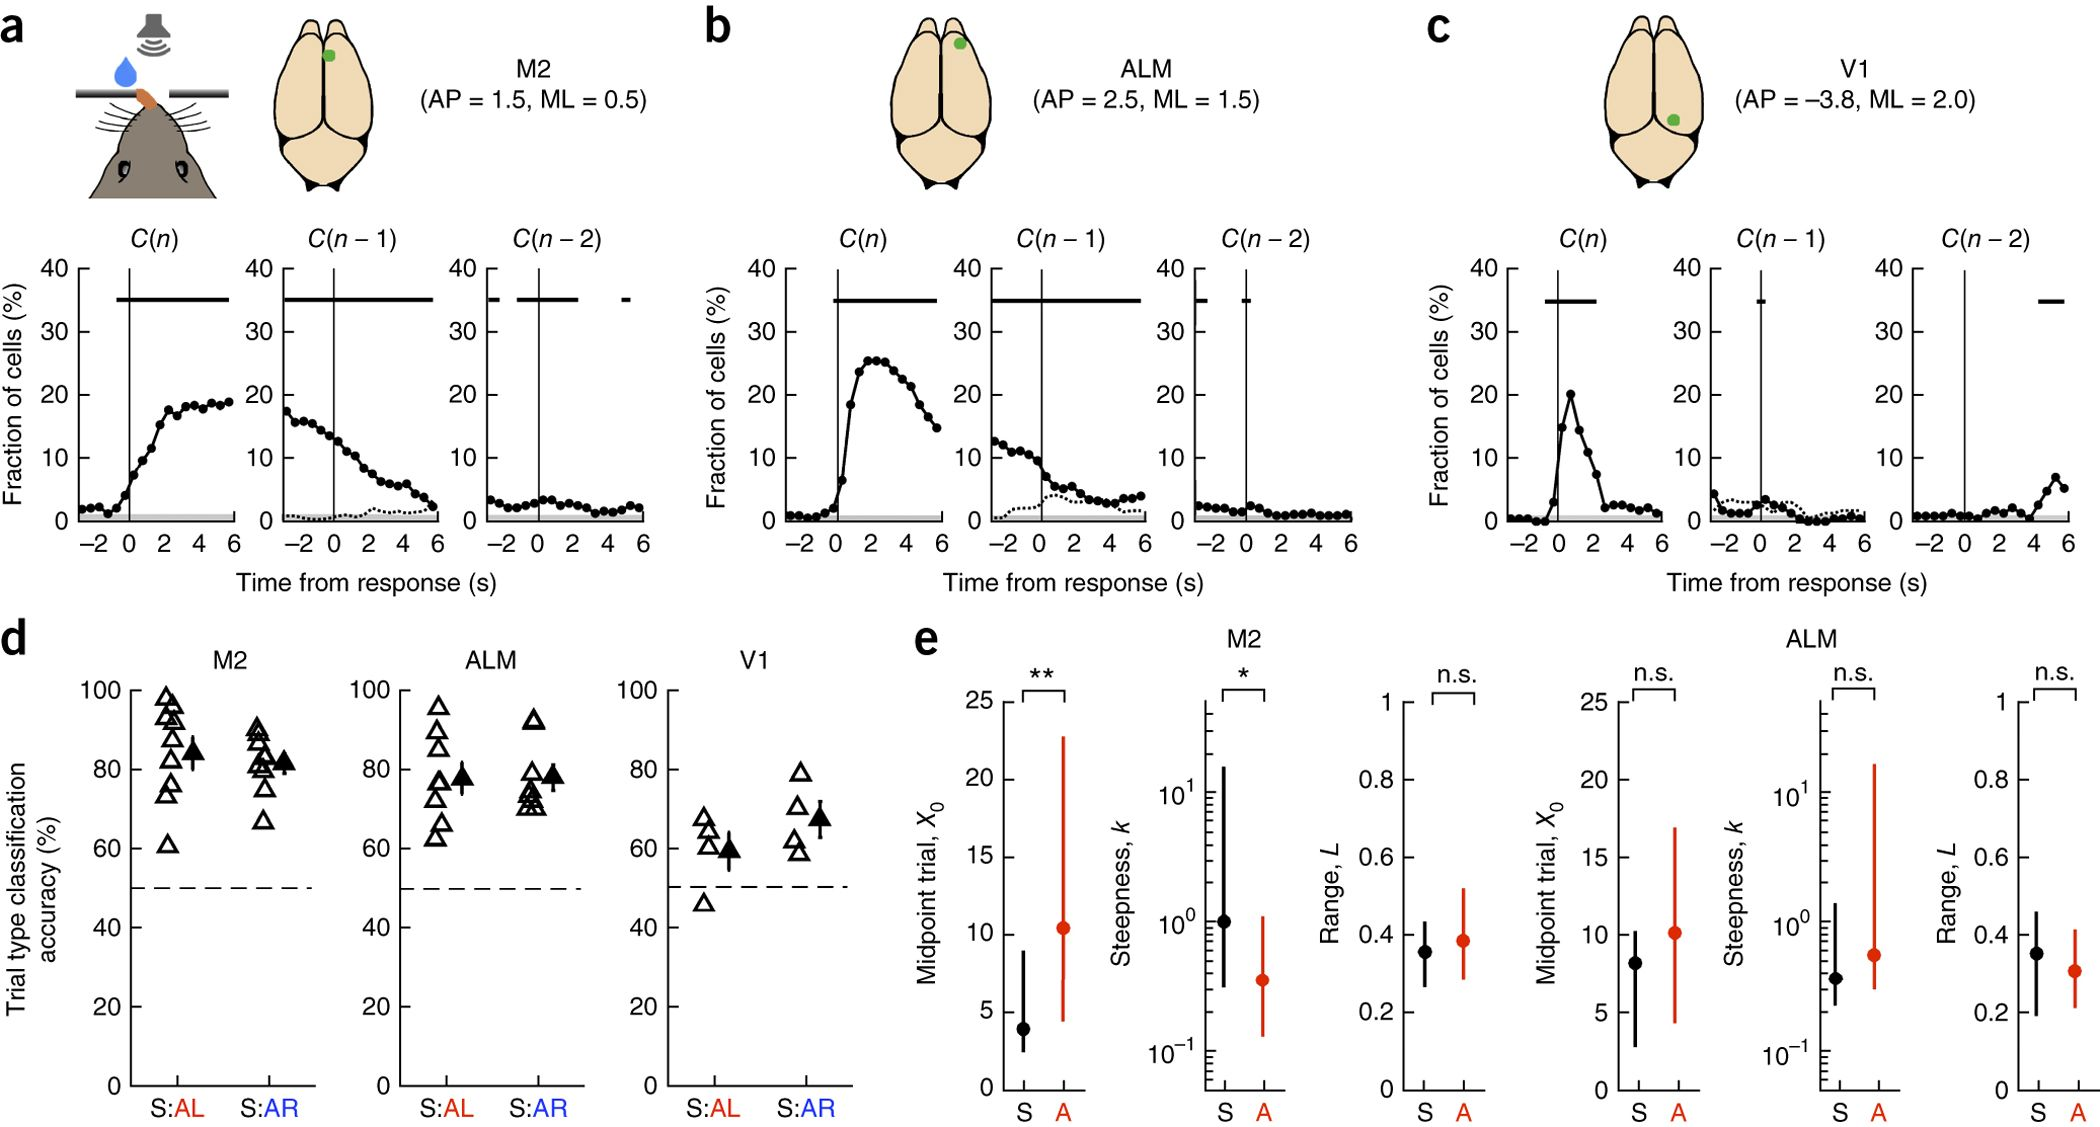
\includegraphics[width=\textwidth]{Figures/Chapter3/NN_fig7} 
\end{center}

\caption[Comparison of neural activity patterns in M2, ALM, and V1]
{
Comparison of neural activity patterns in M2, ALM, and V1 during flexible sensorimotor behavior.
(a) Multiple linear regression analysis was used to evaluate the fraction of 562 M2 neurons encoding choice signals as a function of time. Regression was performed with a moving window ($\mathit{duration} = 0.5$ s, $\mathit{step} = 0.5$ s) to test for significance with $\alpha = 0.01$ on all sound-guided trials where the current and prior choices were rewarded. Black bars, significant fractions ($p < 0.01$, binomial test). Gray shading, significance level of $\alpha=0.01$. Dotted line in the middle panel, fraction of cells significant for the interaction term $C(n) \times C(n-1)$. $N = 9$ sessions from 5 mice. (b) Same as \emph{a} for 518 ALM neurons. $N = 8$ sessions from 4 mice. (c) Same as \emph{a} for 227 V1 neurons. $N = 4$ sessions from 2 mice. (d) Median accuracy of decoding trial type from individual population activity vectors restricted to matched trials, comparing M2, ALM and V1 ensembles. For S:AL, sound or action-left trial types were decoded from trials where the stimulus was an upsweep, choice was left, and outcome was reward for the current trial, and choice was left for the prior trial. For S:AR, sound or action-right trial types were decoded from trials where the stimulus was a downsweep, choice was right, outcome was reward for the current trial, and choice was right for the prior trial. Trial type was decoded with high accuracy using ensemble activity from M2 (matched sound--action-left trials: $84 \pm 4\%$, $t_8 = 8.37$; $p = 3 \times 10^{-5}$; matched sound--action-right trials: $81 \pm 2\%$, $t_8 = 12.73$; $p = 1 \times 10^{-6}$; versus chance level of 50\%, one-sample t-test). Open triangles, individual experiments. Filled triangles, $\mathit{mean}\pm\mathit{SEM}$. Dotted line, chance-level accuracy. (e) Neural transition parameters obtained by fitting action-to-sound (black) and sound-to-action (red) transitions with the logistic function, comparing M2 and ALM ensembles. Wilcoxon rank-sum test, sound vs. action, M2: midpoint trial $x_0$, $p = 0.007$, $z = 2.70$; steepness $k$, $p = 0.03$, $z = -2.17$; height $L$, $p = 0.8$, $z = 0.28$; ALM: $x_0$, $p = 0.11$, $z = 1.62$; $k$, $p = 0.4$, $z = 0.89$; $L$, $p = 0.51$, $z = -0.65$. *$p < 0.05$; **$p < 0.01$; n.s., not significant. Filled circles, medians. Lines end at 25th and 75th percentiles.
}

\label{fig:NN_fig7}
\end{figure}

To investigate ensemble activity, we employed the same dPCA and linear classifier analyses used for M2. We found that rule type could be decoded with high accuracy using ensemble activity from ALM (matched sound, action-left trials: $78 \pm 4\%$, $t(7) = 6.94$; $p = 2 \times 10^{-4}$; matched sound, action-right trials: $78 \pm 3\%$, $t(7) = 8.68$; $p = 5 \times 10^{-5}$; versus chance level of 50\%, one-sample t-test; Fig. \ref{fig:NN_fig7}d), but at a much worse rate for V1 (matched sound, action-left trials: $58 \pm 5\%$, $t(3) = 1.88$; $p = 0.2$; matched sound, action-right trials: $67 \pm 4\%$, $t(3) = 3.76$; $p = 0.03$). Therefore, both ALM and M2 exhibited task-specific ensemble activity patterns. 

However, unlike what we found in M2, characterization of ensemble transitions in ALM did not reveal significant differences between switches to sound versus action blocks (sound: $x_0 = 8.2$, action: $x_0 = 10.2$, median; $z = 1.62$, $p = 0.11$; sound: $k = 0.37$, action: $k = 0.56$, median; $z = 0.89$, $p = 0.4$; Wilcoxon rank-sum test; Fig. \ref{fig:NN_fig7}e). There were also no detectable timing differences between neural and behavioral transitions in ALM (sound: $p = 0.5$, $z = 0.61$; action: $p = 0.13$, $z = -1.50$; Wilcoxon signed-rank test; neural transition defined as 75\% L). 

Taken together, these data indicate regionally specific ensemble dynamics associated with adaptive behavior.